% Chapter Template

\chapter{Contributions} % Main chapter title

\label{Chapter5} % Change X to a consecutive number; for referencing this chapter elsewhere, use \ref{ChapterX}

%----------------------------------------------------------------------------------------
%	SECTION 1
%----------------------------------------------------------------------------------------

The goal of the master's thesis is to propose suitable consumption profiles for supporting residential building consumption optimization and elderly care management.
To achieve this goal, we propose the following steps.

The first step is to obtain a set of datasets. In our case, this will be UK-DALE, REFIT, ECO, REDD, and iAWE.
All datasets measured electrical energy consumption for residential buildings. 
They include main smart meter data, as well as sub-meter data for each appliance in a dwelling. 
For easier handling datasets will be sliced into 1-hour intervals. 
Slices will be put through a classical learning classifier to demonstrate the ability to automatically identify and classify the appliances.
Data will be then used to generate different daily per appliance usage profiles.

\begin{figure}[h!]
	\centering
	\caption{"Universal normalized daily usage profile for weekend and weekday for a microwave. Superposition of data from 25 homes."}
	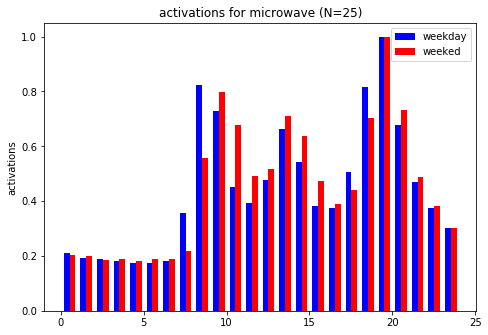
\includegraphics[width=0.9\textwidth]{../Figures/microwave_norm_n25.png}
	\label{fig:UniNormMicrowave}
\end{figure}

One such example can be seen in figure 5. The histogram shows normalized daily 
activation for microwaves. It consists of data from 25 homes from 4 different
datasets. 

During this thesis, more profiles will be presented, using various histogram buckets, dimensions and parameters. 
Each profile presents data from a different perspective, therefore each profile will have a use case of its own.

A table of existing load profiles will be made. It will enable us to place proposed profiles on a map, and possibly 
discover new ways to portray load profiles.

Finally, to demonstrate the usage of developed profiles a demo will be presented. 


